% !TEX TS-program = lualatex

\documentclass[a4paper, 12pt]{article} 

%%%%%%%%%%%%%%%%%
% Fonts, margins etc
%%%%%%%%%%%%%%%%%

\usepackage{fontspec}
%    \defaultfontfeatures{Ligatures={TeX}}

\usepackage{libertine}    %Use Linux Libertine font
    \AtBeginDocument{\addfontfeatures{Ligatures=Historic}}
%\usepackage[libertine]{newtxmath}
%\usepackage{unicode-math}   %Has issues with amsmath
%\setmathfont{Asana-Math}

\usepackage[english]{selnolig}   %Disable ligatures where necessary
    \nolig{st}{s|t}
    
\usepackage[normalem]{ulem} %For underlining
\usepackage{microtype} %Making typesetting even better!
    
\usepackage[usenames,dvipsnames, table]{xcolor} %Add extra colors
%\usepackage[showframe,pass]{geometry}   %Margins
\usepackage[pass]{geometry}   %Margins
%\usepackage[top=2.5cm, bottom=2.5cm, right=2.5cm, left=2.5cm]{geometry}

%%%%%%%%%%%%%%%%%
% Figures
%%%%%%%%%%%%%%%%%  

\usepackage{graphicx} %For importing figures
\usepackage{wrapfig} %For adding figures in text
\usepackage[small,bf]{caption} %Change the format of figure captions
    \captionsetup[subfigure]{format=hang} %And subfigure captions
\usepackage[subrefformat=parens,labelformat=parens]{subfig} %For adding subfigures

%%%%%%%%%%%%%%%%%
%Hyperref package and commands
%%%%%%%%%%%%%%%%%
\usepackage[linktocpage=true, colorlinks=true, citecolor=OliveGreen, linkcolor=OliveGreen, urlcolor=blue]{hyperref}
%Define a command that makes the whole of 'figure 6' a link, not just the number
%Takes two command, e.g. \Ref[figure]{label}
\newcommand*{\Ref}[2][]{\hyperref[#2]{#1~\ref*{#2}}}
%This creates a link to a subfigure e.g. 'Panel (b)'
\newcommand*{\SubRef}[2][]{\hyperref[#2]{#1~\subref{#2}}}

%%%%%%%%%%%%%%%%%
%Bibliography
%%%%%%%%%%%%%%%%%
\usepackage[sorting=none, citestyle=numeric-comp, firstinits=true, 
isbn=false, url=false, doi=false, eprint=false, backend=biber]{biblatex}  
%No sorting means display in citation order, numeric-comp does e.g. [1-4]
%Rest are formatting for actual bibliography
\bibliography{../../Papers.bib}
% Clear notes from references - don't need to be printed
\AtEveryBibitem{\clearfield{note}}
%Make new command for a superscript citation with brackets
%super-b-cite ...
\newcommand*{\superbcite}[1]{$^{[}$\supercite{#1}$^{]}$}

%%%%%%%%%%%%%%%%%
%Tikz packages and modules
%%%%%%%%%%%%%%%%%
\usepackage{tikz}

  %Various tikz libraries
  \usetikzlibrary{matrix} 
  \usetikzlibrary{calc} 
  \usetikzlibrary{positioning}
  \usetikzlibrary{shapes}
  \usetikzlibrary{shapes.multipart}
  \usepgflibrary{shapes.misc}
  \usetikzlibrary{arrows}
  %New command used when overlaying
  \newcommand{\tikzmark}[1]{\tikz[overlay, remember picture] \coordinate (#1);} 
  
%%%%%%%%%%%%%%%%%
% Title formatting
%%%%%%%%%%%%%%%%%  
\usepackage{titling}                      %Titles

%Format the title
\pretitle{\begin{flushleft}\LARGE\bfseries \biolinum}%\addfontfeatures{Ligatures=Historic}}
\posttitle{\par\end{flushleft}}
\preauthor{\begin{flushleft}\large \biolinum}%\addfontfeatures{Ligatures=Historic}}
\postauthor{\end{flushleft}}
\predate{\biolinum}%\addfontfeatures{Ligatures=Historic}}
\postdate{}

%Adjust title spacing
\setlength{\droptitle}{-4em}

% Define the title 
\author{Sam Harrison \hfill \today}
\title{Voxelwise fMRI Node Simulations \\[2pt] \Large Specification File}
\date{}
  
%%%%%%%%%%%%%%%%%
% Section header formatting
%%%%%%%%%%%%%%%%%  
\usepackage[compact]{titlesec}    %Sections

%Modify the titleformat so sections are printed in blue
%Equivalent format to using \usepackage[small]{titlesec}
\titleformat*{\section}{\normalfont\large\bfseries\color{MidnightBlue}}%\addfontfeatures{Ligatures=Historic}}
\titleformat*{\subsection}{\normalfont\normalsize\bfseries\color{MidnightBlue}}%\addfontfeatures{Ligatures=Historic}}
\titleformat*{\subsubsection}{\normalfont\normalsize\bfseries\color{MidnightBlue}}%\addfontfeatures{Ligatures=Historic}}

%Change caption spacing slightly
%\addtolength{\belowcaptionskip}{-1em}

%%%%%%%%%%%%%%%%%
% Header and footer
%%%%%%%%%%%%%%%%%
\usepackage{fancyhdr}

% Format header and footer
\setlength{\headheight}{15.2pt}
\pagestyle{fancyplain}

% Redefine the plain style
\fancypagestyle{plain}{
\fancyhf{} % clear all header and footer fields
\fancyfoot[C]{\thepage} % except the center
\fancyhead[R]{\textcolor{MidnightBlue}{fMRI Simulations}}
\renewcommand{\headrulewidth}{0.4pt}
\renewcommand{\footrulewidth}{0pt}}

% And the normal page style
\rhead{\fancyplain{}{\textcolor{MidnightBlue}{fMRI Simulations}}}
\lhead{}

%%%%%%%%%%%%%%%%%
% Maxwidth command for figures (especially in 2 column environments)
%%%%%%%%%%%%%%%%%

%Defines the \maxwidth command
\makeatletter
\def\maxwidth{%
 \ifdim\Gin@nat@width>\linewidth
  \linewidth
 \else
  \Gin@nat@width
 \fi
}
\makeatother

%%%%%%%%%%%%%%%%%
% Command for a quote environment with an author
%%%%%%%%%%%%%%%%%

%Syntax is:
%\begin{aquote}{Author}
% Quote
%\end{aquote}
\def\signed #1{{\leavevmode\unskip\nobreak\hfil\penalty50\hskip2em
  \hbox{}\nobreak\hfil #1 %
  \parfillskip=0pt \finalhyphendemerits=0 \endgraf}}

\newsavebox\mybox
\newenvironment{aquote}[1]
  {\savebox\mybox{#1}\begin{quote}}
  {\signed{\usebox\mybox}\end{quote}}
  
%%%%%%%%%%%%%%%%%
% Change figure captions for supplementary material
%%%%%%%%%%%%%%%%%
  
  %Change figure name
%\renewcommand{\figurename}{Supplementary figure}
%And number
%\renewcommand{\thefigure}{S\arabic{figure}}


%%%%%%%%%%%%%%%%%
% Maths, algorithms, tables etc
%%%%%%%%%%%%%%%%%  

\usepackage{amsmath} %Generic improvements to math mode e.g. define new \sin, \lim etc
    \DeclareMathOperator{\const}{const}
\usepackage{amssymb} %Extra mathematical symbols e.g.\mathbb{ }
%\usepackage{amsthm}    %Mathematical theorems
%\usepackage{bm}            %Bold mathematical symbols
\usepackage{pdflscape} %Allow pages to be landscape within a portrait document
\usepackage[ruled,lined]{algorithm2e} %For adding pseudocode algorithms
\usepackage{multirow}   %For rows in tables

\usepackage[math-style=ISO, bold-style=ISO]{unicode-math}
    \setmathfont{XITS Math}
    \setmathfont[range=\mathcal]{Latin Modern Math}
    %Latin Modern Math
    %XITS Math
    %Cambria Math
    %Asana Math
    %TeX Gyre Pagella Math
    %%Neo Euler
    \newcommand{\bm}[1]{\mathbf{#1}}

%%%%%%%%%%%%%%%%%%%%%%%%%%%%%%%%%%%%%%%%%%%%%%%%%%%%%%%%%%%%%

\begin{document} 

% Generate the title
\maketitle 

\microtypesetup{protrusion=false} % disables protrusion locally in the document
\tableofcontents % prints Table of Contents
\microtypesetup{protrusion=true} % enables protrusion

\newpage

%%%%%%%%%%%%%%%%%%%%%%%%%%%%%%%%%%%%%%%%%%%%%%%%

\section{Modular Workflow}
\label{sec:Workflow}
We define a `node' as a set of co-activating regions with a common neural\footnote{Neural is taken to mean the activity before HRF convolution.} time course.
There will be a number of these nodes activating and interacting over the course of any fMRI scan.
The fundamental node equation to infer is
\begin{equation}
\bm{D}^{(sr)} = h\big( \bm{P}^{(s)} \bm{A}_{n}^{(sr)} \big) + \bm{\varepsilon}^{(sr)} \,\, .
\label{eq:Model}
\end{equation}
We wish to test the efficacy of methods that try to recover these nodes from resting state scans, where in general none of the four terms on the right of \Ref[equation]{eq:Model} are known.

The obvious way to simulate data to test these methods is:
\begin{enumerate}

\item{Generate a set of spatial maps (\Ref[section]{sec:Maps})}

\item{Generate a set of neural time courses (\Ref[section]{sec:TimeCourses})}

\item{Convolve the overall neural captivity with an HRF (\Ref[section]{sec:HRF})}

\item{Add noise and confounds (\Ref[section]{sec:Noise})}

\end{enumerate}

\subsection{Two stage approach}
\label{sec:ModeModel}
While the fundamental approach implied by \Ref[equation]{eq:Model} contains the general principles, it may be useful to explicitly consider special cases.
For example, consider the model implied by the TFM approach.
In this case, a high dimensional node parcellation is acquired (usually by sICA, but not necessarily), at which point the second step combines these nodes into \emph{modes}\footnote{The distinction between modes and nodes is usually drawn along the lines of modes spatially overlapping and containing anticorrelations.}.
The equation for this case is
\begin{equation}
\bm{D}^{(sr)} = h\Big( \big( \bm{P}^{(s)} \bm{M}^{(s)} \big) \bm{A}_{n}^{(sr)} \Big) + \bm{\varepsilon}^{(sr)} \,\, .
\label{eq:ModeModel}
\end{equation}

In this case, $\bm{P}^{(s)}$, represents a hard, atlas-based parcellation of the brain, with subject variability arising from registration errors.
This set of nodes is then combined into spatially overlapping modes by the action of $\bm{M}^{(s)}$.

%%%%%%%%%%%%%%%%%%%%%%%%%%%%%%%%%%%%%%%%%%%%%%%%

\section{Spatial Maps}
\label{sec:Maps}
The maps should have the following properties, which should be easy to vary:
\begin{itemize}
\item{Sparsity}
\item{Spatial coherence}
\item{Correlation (and higher order statistics)}
\item{Subject variability}
\item{Registration errors}
\end{itemize}

There also needs to be a way to test atlas based methods. 
Could either map all of the above into a brain space, or perhaps generate an atlas in a purely abstract sense.

%%%%%%%%%%%%%%%%%%
\begin{figure}[htb]
\centering
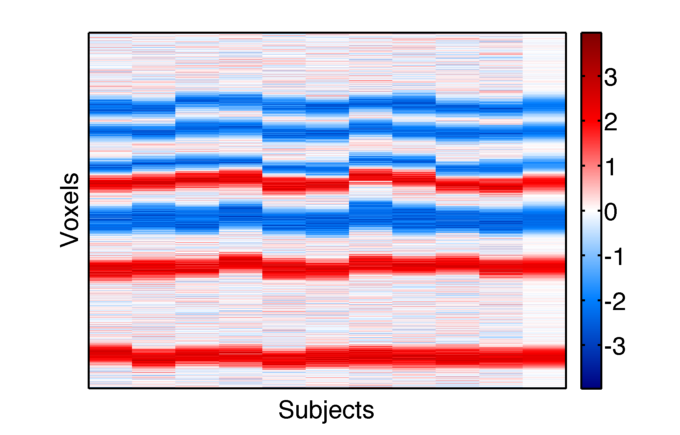
\includegraphics[width=0.9\maxwidth]{Figures/SubjectMaps.png}
\caption{Example of subject variability for one spatial map. The observed maps, including registration errors, are shown for 10 subjects. The mean map, over subjects, is shown on the far right.}
\label{fig:SubjectMaps}
\end{figure}
%%%%%%%%%%%%%%%%%%

\subsection{Two stage node and mode generation}
As described in \Ref[section]{sec:ModeModel}, it may be advantageous to split the spatial maps into a node / mode formulation.
In that case, the properties of the nodes should be:
\begin{itemize}
\item{Binary weights}
\item{Spatial coherence}
\item{Non-overlapping}
\item{Registration errors}
\end{itemize}

Then, the modes need to introduce the properties that are missing compared to the list in \Ref[section]{sec:Maps}.
Therefore, the modes should introduce:
\begin{itemize}
\item{Correlation between modes (and higher order statistics)}
\item{Anti-correlation within modes}
\item{Subject variability}
\end{itemize}

One of the advantages of this formulation is that atlas based methods can be introduced relatively painlessly---the node maps, without the subject misalignments, can form the atlas.

%%%%%%%%%%%%%%%%%%%%%%%%%%%%%%%%%%%%%%%%%%%%%%%%

\section{Neural Time Courses}
\label{sec:TimeCourses}
These represent the neural activity, so should be simulated at a higher sampling rate than TR. 
They should also be simulated for long enough that there are no transient HRF effects (e.g. from zero-padding the convolution). 
Some of the required properties are:
\begin{itemize}
\item{Non-Gaussianity}
\item{Correlation}
\item{Non-stationarity}
\item{Coloured spectra}
\item{Presence / absence in subjects---c.f. left / right lateralised language}
\end{itemize}

%%%%%%%%%%%%%%%%%%%%%%%%%%%%%%%%%%%%%%%%%%%%%%%%

\section{HRF Convolution}
\label{sec:HRF}
This operates on the voxelwise neural activity, and the following should be available, computation permitting:
\begin{itemize}
\item{Linear / nonlinear}
\item{Subject / spatial variability}
\item{Spatio-temporal structure?}
\item{High frequency BOLD?}
\end{itemize}

%%%%%%%%%%%%%%%%%%%%%%%%%%%%%%%%%%%%%%%%%%%%%%%%

\section{Noise \& Confounds}
\label{sec:Noise}
This is simply added to the `clean' BOLD signal generated in the previous steps. 
The simplest model would be spatially and temporally white noise, but some of the following might be useful to include:
\begin{itemize}
\item{Temporal / spatial structure}
\item{Non-Gaussianities}
\item{Voxelwise variance changes}
\item{Interaction with BOLD signal e.g. noise power modulated by signal power}
\item{Physiological confounds---aliased cardiac, very low frequency drifts etc}
\item{Global signal}
\item{Artefactual nodes e.g. motion, multiband etc}
\end{itemize}

%%%%%%%%%%%%%%%%%%%%%%%%%%%%%%%%%%%%%%%%%%%%%%%%

\section{Pre-processing}
\label{sec:Preprocessing}
Want to simulate the standard pre-processing pipeline, so de-meaning, variance normalisation, high-pass filtering etc. 
Could also investigate less common procedures e.g. global signal regression.

Could also investigate different concatenation approaches for methods that assume that.

%%%%%%%%%%%%%%%%%%%%%%%%%%%%%%%%%%%%%%%%%%%%%%

\section{Scoring}
\label{sec:Accuracy}
In the case of a nonlinear HRF there is not an obvious ground truth for methods that infer a linear decomposition. 
The best case is probably the set of subject maps (including registration errors).
The ground truth time courses should probably be just taken as the spatial maps regressed out of the clean BOLD signal.

A complementary scoring mechanism might be the accuracy in separating the BOLD signal from the noise (which is say what the PCA step before an ICA decomposition aims to do).
Again, it's hard to formulate what a good comparison between an atlas method and say ICA would be---this possibly relies on the ability to separate the signal from the noise. 

Maybe a sensible question to ask with these various methods is: do all the voxels within the spatial map contain the same BOLD time course, whatever that may be?

%%%%%%%%%%%%%%%%%%%%%%%%%%%%%%%%%%%%%%%%%%%%%%

\printbibliography

%%%%%%%%%%%%%%%%%%%%%%%%%%%%%%%%%%%%%%%%%%%%%%

\end{document}

  